
\documentclass[aspectratio=169,10pt]{beamer}

\usetheme{Madrid}
\usecolortheme{default}

\usepackage{amsmath}
\usepackage{booktabs}
\usepackage{pgfpages}
\usepackage{tikz}

% Speaker notes:
% Uncomment for slides and notes side by side.
% \setbeameroption{show notes on second screen=right}

\setbeamertemplate{navigation symbols}{}
\setbeamertemplate{footline}[frame number]

\title[Research Progress]{Toward Reliable Consensus\\in Multi-Agent LLM Systems}
\subtitle{Research Direction Exploration}
\author{Your Name}
\institute{Graduate Research Meeting}
\date{October 9, 2026}

\begin{document}

%========================================
% Slide 1
%========================================
\begin{frame}
\titlepage

\note{
Today, I will present my research progress.

My main research area is distributed systems,
especially fault tolerance and consensus.

Recently, I have been exploring how these
concepts can be connected to multi-agent
large language model systems.

Today, I will summarize the papers I have studied,
the problems I identified, and my current
research direction.
}
\end{frame}

%========================================
% Slide 2
%========================================
\begin{frame}{Research Motivation}

\begin{center}
\Large
\textbf{Distributed Systems}
\\[0.3cm]
$\times$
\\[0.3cm]
\textbf{Multi-Agent LLMs}
\end{center}

\vspace{0.5cm}

\begin{block}{Main Question}
How can multiple LLM agents make
reliable collective decisions?
\end{block}

\note{
My motivation is to investigate reliable
decision-making among multiple LLM agents.

LLM agents can produce different answers
even when they receive the same question.

This is different from traditional deterministic
distributed processes.

I want to investigate whether distributed
systems concepts such as agreement,
validity, and fault tolerance can help
improve the reliability of multi-agent systems.
}
\end{frame}

%========================================
% Slide 3
%========================================
\begin{frame}{Papers Studied}

\begin{enumerate}
\setlength{\itemsep}{0.45cm}

\item \textbf{The Byzantine Generals Problem}
\\
{\small Lamport et al., 1982}

\item \textbf{Tight Bound on Mobile Byzantine Agreement}
\\
{\small Bonnet et al., DISC 2014}

\item \textbf{Robust Multi-Agent LLMs under Byzantine Faults}
\\
{\small Recent work under investigation}

\end{enumerate}

\note{
First, I studied The Byzantine Generals Problem
by Lamport and his coauthors.

This paper introduces fundamental agreement
and validity requirements under Byzantine faults.

Second, I studied Tight Bound on Mobile Byzantine
Agreement by Bonnet, Defago, and their coauthors.

This paper considers malicious agents that
move between processes.

Third, I started investigating recent work
on Byzantine robustness in multi-agent LLM systems.

The main purpose is to understand the difference
between classical consensus guarantees
and empirical improvements in LLM reliability.
}
\end{frame}

%========================================
% Slide 4
%========================================
\begin{frame}{Classical Byzantine Agreement}

\begin{center}
\Large
\[
\boxed{\text{Agreement}}
\qquad
\boxed{\text{Validity}}
\qquad
\boxed{\text{Termination}}
\]
\end{center}

\vspace{0.6cm}

\begin{itemize}
\setlength{\itemsep}{0.3cm}
\item Agreement: Same decision
\item Validity: Decision respects initial values
\item Termination: Eventually decide
\end{itemize}

\note{
In classical Byzantine agreement,
three properties are important.

Agreement means that correct processes
must not decide different values.

Validity connects the decision to
the initial values.

Termination means that correct processes
eventually decide.

The exact validity condition depends
on the agreement problem.

For example, in Bonnet's paper,
if all initially correct processes propose
the same value, the decided value must
be that value.

However, validity does not necessarily
mean that the value is factually correct.

This distinction becomes important
when considering LLM-generated answers.
}
\end{frame}

%========================================
% Slide 5
%========================================
\begin{frame}{Mobile Byzantine Agreement}

\begin{center}
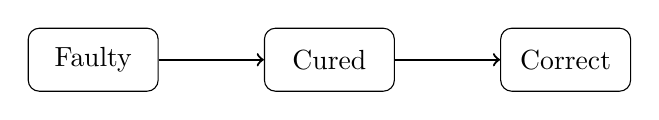
\begin{tikzpicture}[
node distance=1.8cm,
every node/.style={
draw, rounded corners,
minimum width=1.65cm,
minimum height=0.8cm,
align=center
}
]

\node (a) at (0,0) {Faulty};
\node (b) at (3,0) {Cured};
\node (c) at (6,0) {Correct};

\draw[->,thick] (a) -- (b);
\draw[->,thick] (b) -- (c);

\end{tikzpicture}
\end{center}

\vspace{0.6cm}

\begin{center}
\Large
\[
\boxed{n \geq 5t+1}
\]
\end{center}

\begin{itemize}
\item Mobile faults
\item Corrupted internal states
\item Agreement maintenance
\end{itemize}

\note{
Bonnet and his coauthors studied mobile
Byzantine agreement.

Unlike classical Byzantine faults,
malicious agents can move between processes.

When a malicious agent leaves a process,
the process becomes cured.

A cured process executes the correct algorithm,
but its internal state may still be corrupted.

The paper proves that at least five t plus one
processes are required under its model.

Another important contribution is the distinction
between reaching agreement and maintaining
agreement.

Even after agreement has been achieved,
a malicious agent may move and corrupt
a process's stored decision.

Therefore, the protocol must continuously
maintain agreement.
}
\end{frame}

%========================================
% Slide 6
%========================================
\begin{frame}{A Challenge in Multi-Agent LLMs}

\begin{center}
\Large
\[
\underbrace{[A,A,A,B,B]}_{\text{LLM proposals}}
\]

\vspace{0.4cm}

\[
\text{Majority}=A
\qquad
\text{Correct Answer}=B
\]
\end{center}

\vspace{0.5cm}

\begin{alertblock}{Key Observation}
Agreement does not imply answer correctness.
\end{alertblock}

\note{
This is the main problem I identified
when considering consensus among LLM agents.

Suppose five LLM agents generate answers.

Three agents propose A,
while two agents propose B.

A majority vote would select A.

However, suppose the correct answer is B.

All agents could agree on A,
but the final answer would still be incorrect.

This means that classical agreement
and factual correctness are different properties.

Furthermore, a correct LLM process
may produce an incorrect answer
without violating its communication protocol.

Therefore, I think we should distinguish
LLM output uncertainty from Byzantine
protocol deviations.
}
\end{frame}

%========================================
% Slide 7
%========================================
\begin{frame}{Current Research Direction}

\begin{center}

\Large
\textbf{LLM Proposals}

\vspace{0.15cm}
$\downarrow$

\vspace{0.15cm}
\textbf{Deterministic Verification}

\vspace{0.15cm}
$\downarrow$

\vspace{0.15cm}
\textbf{Fault-Tolerant Agreement}

\vspace{0.15cm}
$\downarrow$

\vspace{0.15cm}
\boxed{\text{Verified Decision}}

\end{center}

\note{
My current idea is to separate
LLM reasoning from distributed agreement.

First, multiple LLM agents generate
candidate solutions.

Second, the candidates are checked
using a deterministic verifier.

For example, we could use executable tests,
formal constraints, or proof checking.

Third, distributed processes agree
on a candidate that passes verification.

A digital signature can authenticate
the sender and protect message integrity,
but it cannot prove that an answer is correct.

Therefore, verifiable evidence is required.

This is still a research proposal,
not a new protocol or an established result.

There is already research on validated
Byzantine agreement, so I need to identify
what new problem is introduced by
LLM-generated proposals.
}
\end{frame}

%========================================
% Slide 8
%========================================
\begin{frame}{Open Questions and Next Steps}

\textbf{Open Questions}

\begin{itemize}
\setlength{\itemsep}{0.2cm}
\item How should validity be defined?
\item How can verification cost be reduced?
\item What guarantees remain under faults?
\end{itemize}

\vspace{0.5cm}

\textbf{Next Steps}

\begin{itemize}
\item Study validated Byzantine agreement
\item Select a verifiable task
\item Design a small prototype
\end{itemize}

\note{
My next step is to investigate
validated Byzantine agreement
and related work on verifiable decisions.

I want to focus on tasks where correctness
can be checked mechanically.

Possible applications include
software security and automated incident response.

However, I do not want to introduce LLMs
into systems where deterministic automation
is already sufficient.

The main research question is whether
we can reduce verification costs while
ensuring that correct processes agree
on a candidate satisfying explicit
verification conditions.

I will first study existing protocols
and then build a small prototype
to evaluate feasibility.

At this stage, the novelty of the idea
has not yet been established.
}
\end{frame}

%========================================
% References
%========================================
\begin{frame}{References}

\footnotesize

\begin{thebibliography}{9}

\bibitem{lamport}
L. Lamport, R. Shostak, and M. Pease.
\newblock The Byzantine Generals Problem.
\newblock ACM TOPLAS, 1982.

\bibitem{bonnet}
F. Bonnet, X. D\'efago, T. D. Nguyen,
and M. Potop-Butucaru.
\newblock Tight Bound on Mobile Byzantine Agreement.
\newblock DISC, 2014.

\bibitem{pbft}
M. Castro and B. Liskov.
\newblock Practical Byzantine Fault Tolerance.
\newblock OSDI, 1999.

\end{thebibliography}

\note{
These are the foundational papers
supporting my current research exploration.

The first two are the main papers
I have studied so far.

Practical Byzantine Fault Tolerance
is included as additional background.

Thank you for listening.
}

\end{frame}

\end{document}
